\chapter{Proposed Methodology}

In the pursuit of developing an automatic story generation framework that leverages event-based and graph-based representations, our proposed methodology is designed to enhance narrative coherence, structural organisation, and long-form storytelling. The system follows a multi-stage pipeline incorporating structured event extraction, graph-based event modelling, sequence generation, and evaluation.

\tikzstyle{startstop} = [rectangle, rounded corners, minimum width=3cm, minimum height=1cm, text centered, draw=black]
\tikzstyle{process} = [rectangle, minimum width=3cm, minimum height=1cm, text centered, draw=black]
\tikzstyle{decision} = [diamond, minimum width=3cm, minimum height=1cm, text centered, draw=black]
\tikzstyle{arrow} = [thick,->,>=stealth]


\begin{figure}[ht]
    \centering
    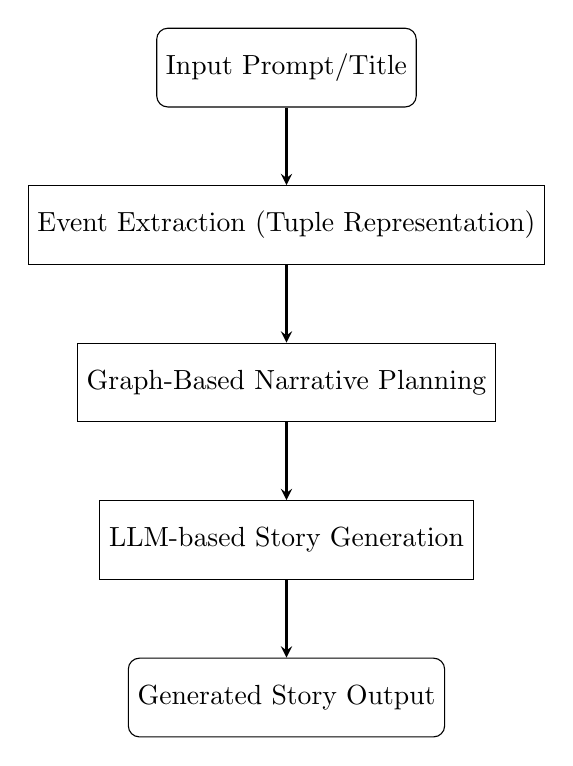
\begin{tikzpicture}[node distance=2cm]
        % Nodes
        \node (input) [startstop] {Input Prompt/Title};
        \node (eventExtraction) [process, below of=input] {Event Extraction (Tuple Representation)};
        \node (graphModeling) [process, below of=eventExtraction] {Graph-Based Narrative Planning};
        \node (llm) [process, below of=graphModeling] {LLM-based Story Generation};
        \node (output) [startstop, below of=llm] {Generated Story Output};

        % Arrows
        \draw [arrow] (input) -- (eventExtraction);
        \draw [arrow] (eventExtraction) -- (graphModeling);
        \draw [arrow] (graphModeling) -- (llm);
        \draw [arrow] (llm) -- (output);
    \end{tikzpicture}
    \caption{Workflow of the Proposed Methodology}
    \label{fig:workflow}
\end{figure}

\section{Event Extraction and Representation}
The foundation of our approach lies in structuring narratives through event-based representation. Events are abstracted from source text using natural language processing techniques, where each event consists of a subject, verb, object, and additional contextual attributes. The extraction process involves:
\begin{itemize}
    \item \textbf{Dependency Parsing}: Utilising syntactic analysis to identify verb-centric event structures from text.
    \item \textbf{Coreference Resolution}: Mapping entities across sentences to maintain continuity and avoid fragmentation.
    \item \textbf{Semantic Role Labelling (SRL)}: Assigning thematic roles to event participants to enhance event understanding.
    \item \textbf{Event Normalisation}: Standardising events to reduce sparsity in learning while preserving semantic richness.
\end{itemize}
These extracted events form structured sequences that facilitate learning patterns in storytelling.

\section{Graph-Based Narrative Planning}
Once events are extracted, a graph-based modelling approach is applied to structure narratives in a logically consistent manner. The graph representation captures relationships between events, characters, and narrative dependencies.
\begin{itemize}
    \item \textbf{Directed Acyclic Graph (DAG) Construction}: Nodes represent events, and edges define logical transitions.
    \item \textbf{Causal and Temporal Dependencies}: Incorporating precedence constraints to maintain event sequencing.
    \item \textbf{Entity Interactions}: Character-centric subgraphs model relationships and dialogue structures.
    \item \textbf{Plot Consistency Checks}: Graph validation ensures coherence by enforcing thematic connections.
\end{itemize}
This graph-based approach facilitates goal-directed story progression, addressing common issues in long-form AI-generated narratives.

\section{Story Generation Model}
With event sequences structured within a graph framework, the story generation process involves translating these representations into natural language text. The methodology employs sequence-to-sequence learning, leveraging pre-trained transformer models with fine-tuned conditioning on event sequences
\begin{itemize}
    \item \textbf{Pre-trained Language Models}: Utilising models such as T5 or GPT architectures adapted for structured narrative generation.
    \item \textbf{Hierarchical Generation}: First generating high-level plot summaries before expanding into detailed text.
    \item \textbf{Event-to-Sentence Transformation}: Converting structured event representations into grammatically coherent sentences.
    \item \textbf{Neural Discourse Planning}: Integrating discourse structures (e.g., causality, sentiment transitions) to enhance readability.
\end{itemize}

\section{Evaluation Metrics and Validation}
Evaluating AI-generated stories remains a complex challenge due to the subjective nature of storytelling quality. Our evaluation framework employs a combination of automatic metrics and human assessments.
\begin{itemize}
    \item \textbf{Automated Metrics}:
    \begin{itemize}
         \item \textbf{BLEU \& ROUGE}: Measuring lexical overlap with reference narratives.
        \item \textbf{BERTScore}: Capturing semantic similarity between generated and human-written stories.
        \item \textbf{Graph Coherence Metric}: Quantifying logical consistency within the event graph.
    \end{itemize}
    \item \textbf{Human Evaluation}:
    \begin{itemize}
         \item \textbf{Narrative Coherence Test}: Evaluators assess structural integrity and logical transitions.
         \item \textbf{Creativity Rubric}: Subjective evaluation based on originality and engagement.
         \item \textbf{Torrance Test for Creative Writing (TTCW)}: Adapted criteria for AI-generated storytelling.
    \end{itemize}
\end{itemize}